%-----------------------------------LICENSE------------------------------------%
%   This file is part of Mathematics-and-Physics.                              %
%                                                                              %
%   Mathematics-and-Physics is free software: you can redistribute it and/or   %
%   modify it it under the terms of the GNU General Public License as          %
%   published by the Free Software Foundation, either version 3 of the         %
%   License, or (at your option) any later version.                            %
%                                                                              %
%   Mathematics-and-Physics is distributed in the hope that it will be useful, %
%   but WITHOUT ANY WARRANTY; without even the implied warranty of             %
%   MERCHANTABILITY or FITNESS FOR A PARTICULAR PURPOSE.  See the              %
%   GNU General Public License for more details.                               %
%                                                                              %
%   You should have received a copy of the GNU General Public License along    %
%   with Mathematics-and-Physics.  If not, see <https://www.gnu.org/licenses/>.%
%------------------------------------------------------------------------------%

% Use the standalone class for displaying the tikz image on a small PDF.
\documentclass[crop, tikz]{standalone}

% Needed for mathbb.
\usepackage{amssymb}

% Import the tikz package to use for the drawing.
\usepackage{tikz}

% Load the arrows.meta library.
\usetikzlibrary{arrows.meta}

% Begin the document.
\begin{document}

    % Draw the figure.
    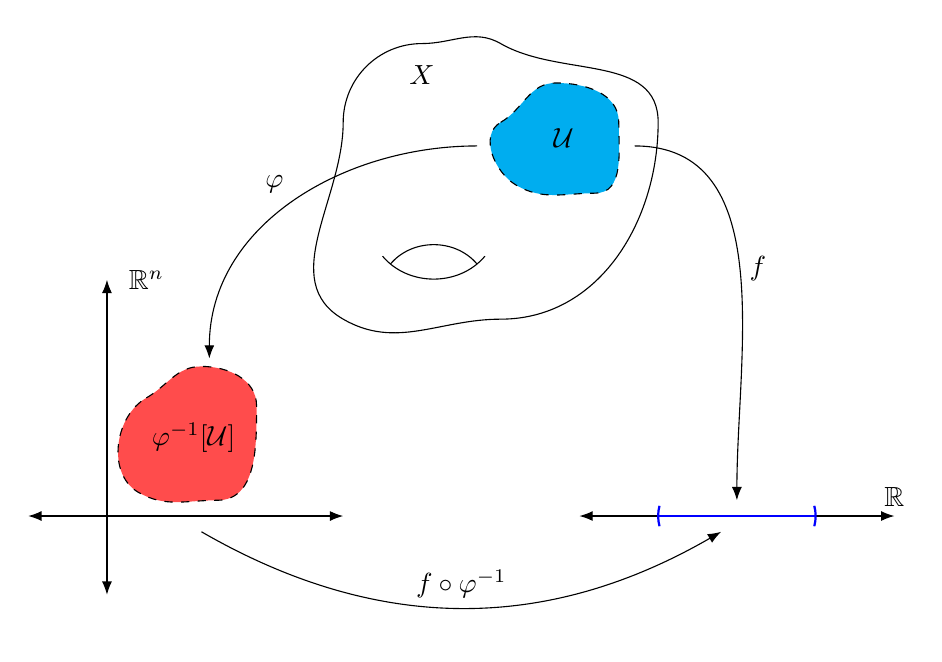
\begin{tikzpicture}[>=LaTeX]
        \draw[<->] (-1,  0) to (3, 0);
        \draw[<->] ( 0, -1) to (0, 3);
        \draw[dashed, fill=red!70!white]
        (0.5, 1.5) to[out=30,  in=180]  (1.2,  1.9)
                   to[out=0,   in=90]   (1.9,  1.4)
                   to[out=-90, in=0]    (1.4,  0.2)
                   to[out=180, in=-30]  (0.4,  0.3)
                   to[out=150, in=-150] cycle;

        \node at (0.5, 3.0) {$\mathbb{R}^{n}$};
        \node at (1.1, 1.0) {$\varphi^{-1}[\mathcal{U}]$};
        \draw[<-]
            (1.3,2) to[out=90, in=180] node[above left] {$\varphi$} (4.7,4.7);

        \begin{scope}[xshift=3cm,yshift=5cm]
            \draw (0,0) to[out=90,  in=180] (1,  1.0)
                        to[out=0,   in=150] (2,  1.0)
                        to[out=-30, in=90]  (4,  0.0)
                        to[out=-90, in=0]   (2, -2.5)
                        to[out=180, in=-30] (0, -2.5)
                        to[out=150, in=-90] cycle;

            \draw (0.5, -1.7) to[in=-130, out=-50] (1.8, -1.7);
            \draw (0.6, -1.8) to[in=130,  out=50]  (1.7, -1.8);

            \draw[dashed, fill=cyan]
                (2.0, 0.0) to[out=30,  in=180]  (2.7,  0.5)
                           to[out=0,   in=90]   (3.5,  0.0)
                           to[out=-90, in=0]    (3.2, -0.9)
                           to[out=180, in=-30]  (2.2, -0.8)
                           to[out=150, in=-150] cycle;

            \node at (2.8, -0.2) {$\mathcal{U}$};
            \node at (1.0,  0.6) {$X$};
        \end{scope}
        \draw[<->] (6, 0) to (10, 0) node[above] {$\mathbb{R}$};
        \draw[->]  (6.7, 4.7) to[out=0, in=90] node[right] {$f$} (8, 0.2);
        \draw[blue, thick] (9, 0) arc (0:15:0.5);
        \draw[blue, thick] (9, 0) arc (0:-15:0.5);
        \draw[blue, thick] (7, 0) arc (180:195:0.5);
        \draw[blue, thick] (7, 0) arc (180:165:0.5);
        \draw[blue, thick] (7,0) to (9, 0);
        \draw[->] (1.2, -0.2) to[out=-30, in=-150]
            node[above] {$f\circ\varphi^{-1}$} (7.8, -0.2);
    \end{tikzpicture}
\end{document}
